
\section{Additional Experimental Results}

\begin{figure}[H]
  \centering
  \subfloat[Wine]{
    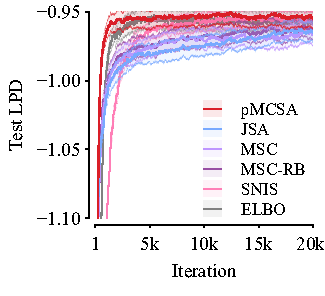
\includegraphics[scale=0.9]{figures/wine_01.pdf}
  }\hspace{0.2in}
  \subfloat[Wine]{
    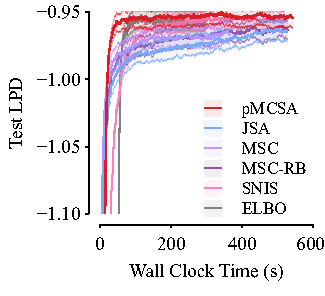
\includegraphics[scale=0.9]{figures/wine_02.pdf}
  } \\
  \subfloat[Concrete]{
    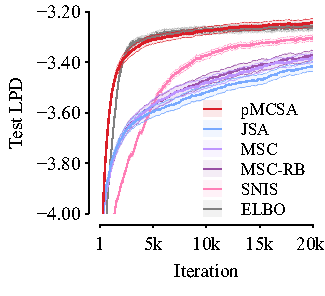
\includegraphics[scale=0.9]{figures/concrete_01.pdf}
  } \hspace{0.2in}
  \subfloat[Concrete]{
    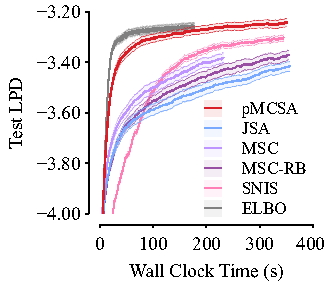
\includegraphics[scale=0.9]{figures/concrete_02.pdf}
  } \\
  \subfloat[Boston]{
    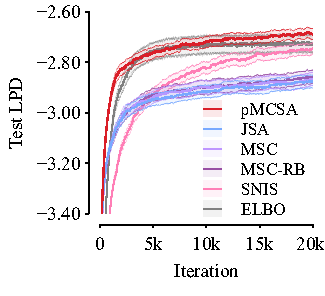
\includegraphics[scale=0.9]{figures/boston_01.pdf}
  }\hspace{0.2in}
  \subfloat[Boston]{
    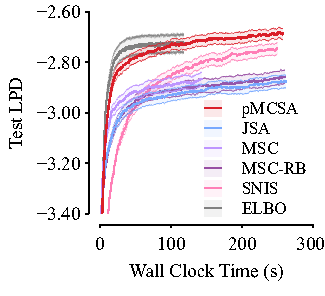
\includegraphics[scale=0.9]{figures/boston_02.pdf}
  } \\
  \subfloat[Yacht]{
    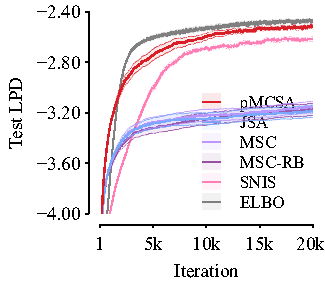
\includegraphics[scale=0.9]{figures/yacht_01.pdf}
  }\hspace{0.2in}
  \subfloat[Yacht]{
    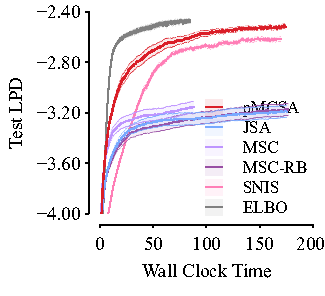
\includegraphics[scale=0.9]{figures/yacht_02.pdf}
  }
  \caption{Bayesian Neural Network Regression}
\end{figure}

%%% Local Variables:
%%% TeX-master: "master"
%%% End:
